%HW1.tex
%
% First Homework for Graduate Algebra
% Frank Sottile
%%%%%%%%%%%%%%%%%%%%%%%%%%%%%%%%%%%%%%%%%%%%%%%%%%%%%%%%%%%%%%%%%%%%%%%
\documentclass[12pt]{article}
\usepackage{multicol,amssymb,amsmath}
\usepackage{graphicx}
\usepackage{xcolor}
\headheight=8pt
%
\topmargin=-95pt
\textheight=744pt   \textwidth=580pt
\oddsidemargin=-60pt \evensidemargin=-60pt

\pagestyle{empty}

%%%%%%%%%%%%%%%%%%%%%%%%%%%%%%%%%%%%%%%%%%%%
\newcommand{\HH}{{\mathbb H}}
\newcommand{\FF}{{\mathbb F}}
\newcommand{\RR}{{\mathbb R}}
\newcommand{\CC}{{\mathbb C}}
\newcommand{\KK}{{\mathbb K}}
\newcommand{\NN}{{\mathbb N}}
\newcommand{\TT}{{\mathbb T}}
\newcommand{\ZZ}{{\mathbb Z}}
\newcommand{\calA}{{\mathcal A}}
\newcommand{\be}{{\bf e}}

\newcommand{\Hom}{\mbox{Hom}}
\newcommand{\spec}{\mbox{spec}}
\newcommand{\cone}{\mbox{cone}}

\newcommand{\Square}{\raisebox{-2pt}{\includegraphics{figures/Square.eps}}}

\newcommand{\vect}[2]{(\begin{smallmatrix}#1\\#2\end{smallmatrix})}
\newcommand{\msp}{\hspace{8pt}}

\newcommand{\barsl}{\noindent\begin{minipage}[t]{575pt}
{\color{violet}\rule{575pt}{1.2pt}}\vspace{-5.7mm}\\
{\color{blue}\rule{575pt}{1.2pt}}\vspace{-5.7mm}\\
{\color{green}\rule{575pt}{1.2pt}}\vspace{-5.7mm}\\
{\color{yellow}\rule{575pt}{1.2pt}}\vspace{-5.7mm}\\
{\color{orange}\rule{575pt}{1.2pt}}\vspace{-5.7mm}\\
{\color{red}\rule{575pt}{1.2pt}}
\end{minipage}}


\def\demph#1{{\color{brown}{\sl #1}}}
\def\defcolor#1{{\color{brown}#1}}

\begin{document}
\LARGE 
\noindent
Algebra II\ \ Winter 2021 \hfill 20 January\makebox[40pt][l]{\ }\\
Frank Sottile \hfill
\Large\sf
Eleventh Homework\makebox[40pt][l]{\ }\\
\large\vspace{5pt}


\noindent
Write your answers neatly, in complete sentences.
Start each problem on a new page (this makes it easier for Gradescope).
Revise your work before handing it in, and submit a .pdf  created from a LaTeX source to Gradescope.
Correct and crisp proofs are greatly appreciated; oftentimes your work can be shortened and made clearer.\newline
\vspace{-5pt}

\barsl

\begin{enumerate}
%%%%%%%%%%%%%%%%%%%%%%%%%%%%%%%%%%%%%
%\setcounter{enumi}{52}

%%%%%%%%%%%%%%%%%%%%%%%%%%%%%%%%%%%%%%%%%%%%%%%%%%%%%%%%%%%%%%%%%%%%%%%%%%%%%%%%%
\item Suppose that $S\subset R$ is a multiplicatively closed subset of an integral domain $R$ that does not contain $0$.
       Prove that if $R$ is a principal ideal domain, then so is $R[S^{-1}]$, and we have the same implication for unique
       factorization domains.
   \vspace{-2pt} 
%%%%%%%%%%%%%%%%%%%%%%%%%%%%%%%%%%%%%%%%%%%%%%%%%%%%%%%%%%%%%%%%%%%%%%%%%%%%%%%%%

%\newpage
%%%%%%%%%%%%%%%%%%%%%%%%%%%%%%%%%%%%%%%%%%%%%%%%%%%%%%%%%%%%%%%%%%%%%%%%%%%%%%%%%
\item Let $R$ be an integral domain, and for each  maximal ideal $\mathfrak{m}$ of $R$, show that the localization
  $R_{\mathfrak m}$ is a subring of the quotient field of $R$.\vspace{-2pt}
%%%%%%%%%%%%%%%%%%%%%%%%%%%%%%%%%%%%%%%%%%%%%%%%%%%%%%%%%%%%%%%%%%%%%%%%%%%%%%%%%


%\newpage
%%%%%%%%%%%%%%%%%%%%%%%%%%%%%%%%%%%%%%%%%%%%%%%%%%%%%%%%%%%%%%%%%%%%%%%%%%%%%%%%%
\item Continuing the previous problem, show that the intersection of the rings $R_{\mathfrak m}$, as ${\mathfrak m}$
  ranges over all maximal ideals of $R$, is $R$ itself.\vspace{-2pt}
%%%%%%%%%%%%%%%%%%%%%%%%%%%%%%%%%%%%%%%%%%%%%%%%%%%%%%%%%%%%%%%%%%%%%%%%%%%%%%%%%


 
%\newpage
%%%%%%%%%%%%%%%%%%%%%%%%%%%%%%%%%%%%%%%%%%%%%%%%%%%%%%%%%%%%%%%%%%%%%%%%%%%%%%%%%
\item Show that the equation $x^2+1=0$ has infinitely many solutions in Hamilton's Quaternions,
       $\HH$, which is $\RR\oplus i\RR\oplus j\RR\oplus k\RR$, where $ij=k$, $ji=-k$, etc.
       These are defined in the Example on page 117 of my copy of Hungerford in Section III.1.\vspace{-2pt}
%%%%%%%%%%%%%%%%%%%%%%%%%%%%%%%%%%%%%%%%%%%%%%%%%%%%%%%%%%%%%%%%%%%%%%%%%%%%%%%%%


%\newpage
%%%%%%%%%%%%%%%%%%%%%%%%%%%%%%%%%%%%%%%%%%%%%%%%%%%%%%%%%%%%%%%%%%%%%%%%%%%%%%%%%
\item Let $F$ be a field, and consider the ring of formal power series $R:=\FF[[x]]$ in one variable.
      Show that $f\in R$ is a unit if and only if it has a nonzero constant term.
       Use this to show that the only ideals in $R$ are $\{ \langle x^n\rangle\mid n\in \NN\}$.\vspace{-2pt}
%%%%%%%%%%%%%%%%%%%%%%%%%%%%%%%%%%%%%%%%%%%%%%%%%%%%%%%%%%%%%%%%%%%%%%%%%%%%%%%%%

%\newpage
%%%%%%%%%%%%%%%%%%%%%%%%%%%%%%%%%%%%%%%%%%%%%%%%%%%%%%%%%%%%%%%%%%%%%%%%%%%%%%%%%
\item Continuing the previous problem, show that the subring $\FF[[x]][x^{-1}]$ of the 
      quotient field of $\FF[[x]]$ is a field.
      This is the field of formal Laurent series in $x$.\vspace{-2pt}
%%%%%%%%%%%%%%%%%%%%%%%%%%%%%%%%%%%%%%%%%%%%%%%%%%%%%%%%%%%%%%%%%%%%%%%%%%%%%%%%%



       
%\newpage
%%%%%%%%%%%%%%%%%%%%%%%%%%%%%%%%%%%%%%%%%%%%%%%%%%%%%%%%%%%%%%%%%%%%%%%%%%%%%%%%%
\item
 (a) If $D$ is an integral domain and $c$ is an irreducible element in $D$, show that $D[x]$ is not a principal ideal domain.
  (Hint: consider the ideal generated by $x$ and $c$.)

  (b) Show that $\ZZ[x]$ is not a principal ideal domain.

  (c) If $\FF$ is a field and $n\geq 2$, show that $\FF[x_1,\dotsc,x_n]$ is not a principal ideal domain.
      (Hint: show that $x_1$ is irreducible in $\FF[x_1,\dotsc,x_{n-1}]$.)
       \vspace{-2pt}
%%%%%%%%%%%%%%%%%%%%%%%%%%%%%%%%%%%%%%%%%%%%%%%%%%%%%%%%%%%%%%%%%%%%%%%%%%%%%%%%%

\end{enumerate}
%%%%%%%%%%%%%%%%%%%%%%%%%%%%%%%%%%%%%%%%%%%%%%%%%%%%%%%%%%%%%%%


\end{document}
